%%%%%%%%%%%%%%%%%%%%%%%%%%%%%%%%%%%%%%%%%
% Beamer Presentation
% LaTeX Template
% Version 1.0 (10/11/12)
%
% This template has been downloaded from:
% http://www.LaTeXTemplates.com
%
% License:
% CC BY-NC-SA 3.0 (http://creativecommons.org/licenses/by-nc-sa/3.0/)
%
%%%%%%%%%%%%%%%%%%%%%%%%%%%%%%%%%%%%%%%%%

%----------------------------------------------------------------------------------------
%	PACKAGES AND THEMES
%----------------------------------------------------------------------------------------

\documentclass{beamer}

\mode<presentation> {

% The Beamer class comes with a number of default slide themes
% which change the colors and layouts of slides. Below this is a list
% of all the themes, uncomment each in turn to see what they look like.

%\usetheme{default}
%\usetheme{AnnArbor}
%\usetheme{Antibes}
%\usetheme{Bergen}
%\usetheme{Berkeley}
%\usetheme{Berlin}
%\usetheme{Boadilla}
%\usetheme{CambridgeUS}
%\usetheme{Copenhagen}
%\usetheme{Darmstadt}
%\usetheme{Dresden}
%\usetheme{Frankfurt}
%\usetheme{Goettingen}
%\usetheme{Hannover}
%\usetheme{Ilmenau}
%\usetheme{JuanLesPins}
%\usetheme{Luebeck}
\usetheme{Madrid}
%\usetheme{Malmoe}
%\usetheme{Marburg}
%\usetheme{Montpellier}
%\usetheme{PaloAlto}
%\usetheme{Pittsburgh}
%\usetheme{Rochester}
%\usetheme{Singapore}
%\usetheme{Szeged}
%\usetheme{Warsaw}

% As well as themes, the Beamer class has a number of color themes
% for any slide theme. Uncomment each of these in turn to see how it
% changes the colors of your current slide theme.

%\usecolortheme{albatross}
%\usecolortheme{beaver}
%\usecolortheme{beetle}
%\usecolortheme{crane}
%\usecolortheme{dolphin}
%\usecolortheme{dove}
%\usecolortheme{fly}
%\usecolortheme{lily}
%\usecolortheme{orchid}
%\usecolortheme{rose}
%\usecolortheme{seagull}
%\usecolortheme{seahorse}
%\usecolortheme{whale}
%\usecolortheme{wolverine}

%\setbeamertemplate{footline} % To remove the footer line in all slides uncomment this line
%\setbeamertemplate{footline}[page number] % To replace the footer line in all slides with a simple slide count uncomment this line

%\setbeamertemplate{navigation symbols}{} % To remove the navigation symbols from the bottom of all slides uncomment this line
}

\usepackage{graphicx} % Allows including images
\usepackage{booktabs} % Allows the use of \toprule, \midrule and \bottomrule in tables
\usepackage[absolute,overlay]{textpos}
\setbeamercolor{framesource}{fg=gray}
\setbeamerfont{framesource}{size=\tiny}
\newcommand{\source}[1]{
\begin{textblock*}{6cm}(0.1cm,8.7cm)
    \begin{beamercolorbox}[ht=0.5cm,left]{framesource}
        \usebeamerfont{framesource}\usebeamercolor[fg]{framesource} Image Source: {#1}
    \end{beamercolorbox}
\end{textblock*}}
%----------------------------------------------------------------------------------------
%	TITLE PAGE
%----------------------------------------------------------------------------------------

\title[MVCNN \& LSTM for Screening Challenge]{Passanger Screening Challenge using MVCNN \& LSTM} % The short title appears at the bottom of every slide, the full title is only on the title page

\author{Yuyang Rong, Peng Ding} % Your name
\institute[SIST] 
% Your institution as it will appear on the bottom of every slide, may be shorthand to save space
{
School of Information Science and Technology(SIST) \\
Shanghaitech University \\ % Your institution for the title page
\medskip
\textit{\{rongyy, dingpeng\}@shanghaitech.edu.cn} % Your email address
}
\date{\today} % Date, can be changed to a custom date

\begin{document}

\begin{frame}
\titlepage % Print the title page as the first slide
\end{frame}

\begin{frame}
\frametitle{Overview} % Table of contents slide, comment this block out to remove it
\tableofcontents % Throughout your presentation, if you choose to use \section{} and \subsection{} commands, these will automatically be printed on this slide as an overview of your presentation
\end{frame}

%----------------------------------------------------------------------------------------
%	PRESENTATION SLIDES
%----------------------------------------------------------------------------------------

%------------------------------------------------
\section{Introduction} % Sections can be created in order to organize your presentation into discrete blocks, all sections and subsections are automatically printed in the table of contents as an overview of the talk
%------------------------------------------------

\begin{frame}
\frametitle{Introduction: Motivation}
	\begin{itemize}
	\item Is any passenger carrying dangerous objects? If so, where are the objects?
	\item Transportation Security Administration(TSA): Use Millimeter Wave Unit to find out
	\item The image can be vague and unclear.
	\item Humans is not efficient in determining whether a passenger is carrying banned object.
	\item \textbf{How can machines help?}
	\end{itemize}
	\begin{figure}
		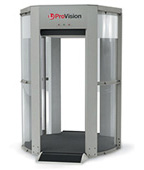
\includegraphics[width=2cm]{../Pic/MillimeterWaveUnit.jpg}
		\caption{Millimeter Wave Unit}
	\end{figure}
	\source{https://en.wikipedia.org/wiki/Millimeter\_wave\_scanner}
\end{frame}

%------------------------------------------------
\section{Problem Statement} % Sections can be created in order to organize your presentation into discrete blocks, all sections and subsections are automatically printed in the table of contents as an overview of the talk
%------------------------------------------------

\begin{frame}
\frametitle{Problem Statement}
	\begin{itemize}
	\item Let's talk about humans first.
	\item Even if someone is carrying forbidden objects, how to tell where it is?
	\item We define 17 regions out of human body.
	\end{itemize}
	\begin{figure}
		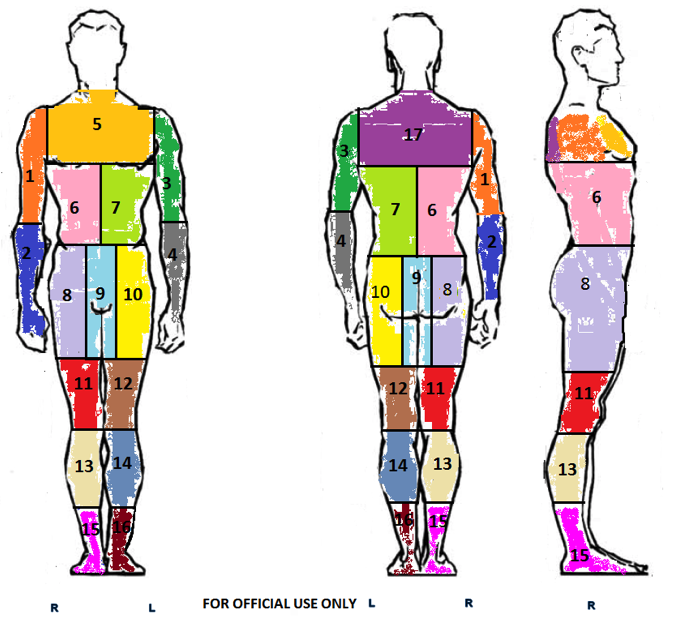
\includegraphics[width=6cm]{../Pic/body_zones.png}
		\caption{Region Definition}
	\end{figure}
	\source{TSA: Definition}
\end{frame}
%------------------------------------------------
\begin{frame}
\frametitle{Problem Statement}
	\begin{itemize}
		\item Given a consecutive images of one person from 16 different angles with labels of 17 regions.
		\item Train a network to predict if there is dangerous object in each of 17 regions.
	\end{itemize}
\end{frame}
%------------------------------------------------

\begin{frame}
\frametitle{Problem Statement}
	\begin{figure}
		\centering
		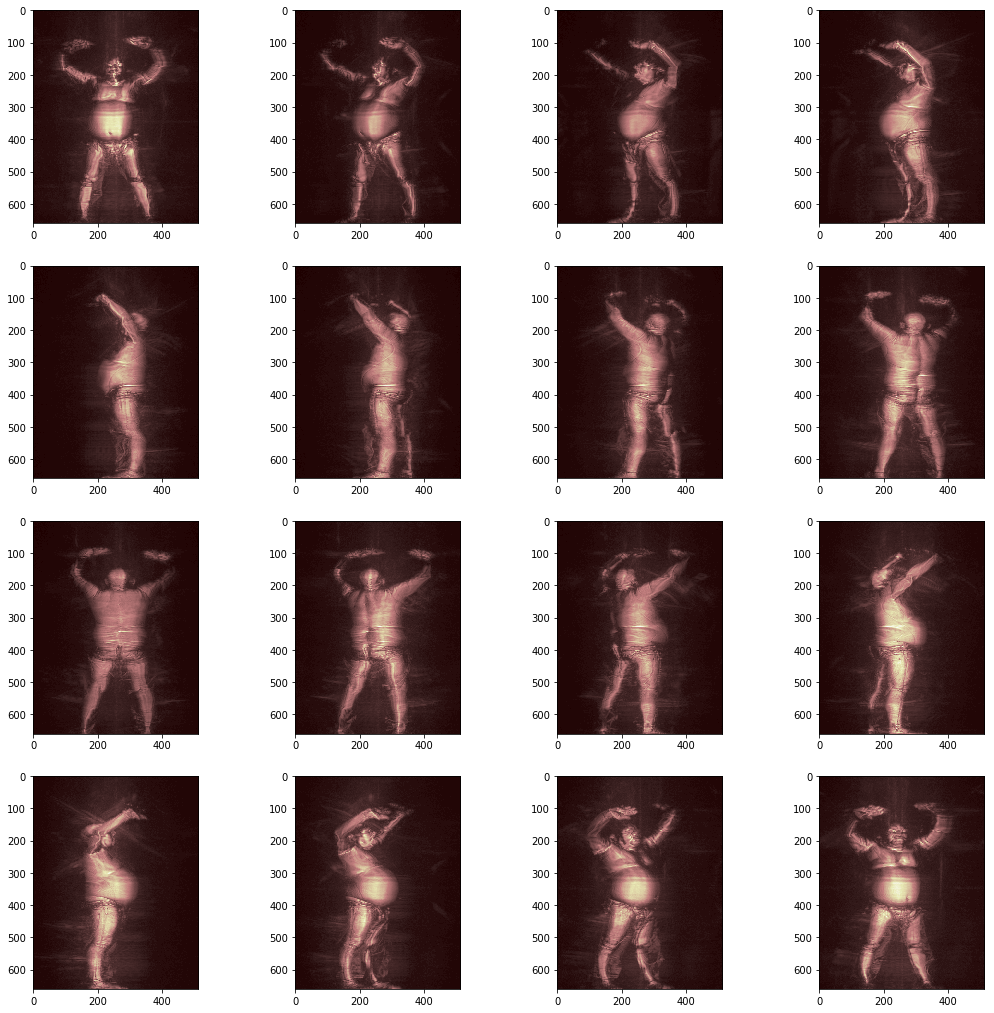
\includegraphics[width=6cm]{../Pic/ffefec0cd4e1e2c3fe64bb93f082efdd.png}
		\caption{16 Images of a same person from different angles.}
	\end{figure}	
	\source{TSA: Dataset}
\end{frame}

%------------------------------------------------

\section{Difficulties}
\begin{frame}
\frametitle{Difficulties}
	\begin{itemize}
		\item No or little feature and Noise, even human cannot label it well.
		\item Broken and rigged data: Not all regions are labeled.
		\item Not much positive labels. Of 1k people and 10k labels, only about 1k positive labels
		\item The file is too big. Low resolution images(listed above) takes 10M per person.
	\end{itemize}
\end{frame}

\begin{frame}
\frametitle{Difficulties: Noisy Data}
	\begin{figure}
		\centering
		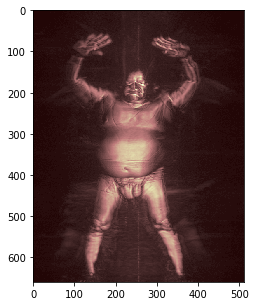
\includegraphics[width=5cm]{../Pic/noisy.png}
		\caption{This person is labeled to have dangerous objects in his right arm and crotch}
	\end{figure}	
	\source{TSA: Dataset}
\end{frame}

\begin{frame}
\frametitle{Difficulties: Rigged Data}
	\begin{figure}
		\centering
		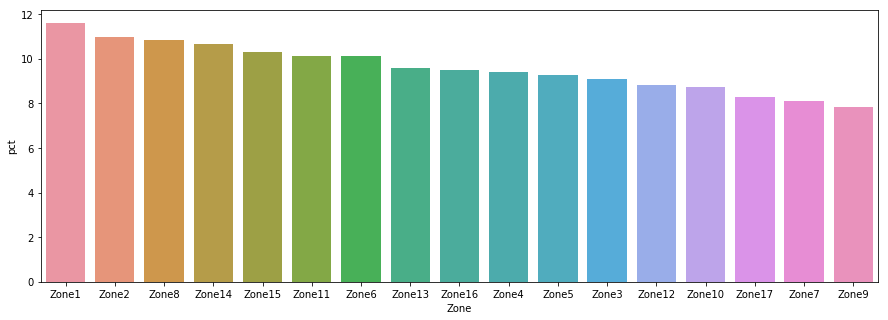
\includegraphics[width=10cm]{../Pic/bars.png}
		\caption{The most popular to hide things is your right arm and the least popular one is crotch?}
	\end{figure}	
\end{frame}


%------------------------------------------------
\section{Out Approach} % Sections can be created in order to organize your presentation into discrete blocks, all sections and subsections are automatically printed in the table of contents as an overview of the talk
%------------------------------------------------

%------------------------------------------------
\begin{frame}
\frametitle{Our Approach: Crop \& PCA}
	\begin{itemize}
		\item Crop each image and put the same region together.
		\item Black background is suitable for PCA
		\item Problem: Not every region is shown in a certain image.
		\item Problem: Have to train 17 models for 17 regions...
	\end{itemize}
	\begin{figure}
		\centering
		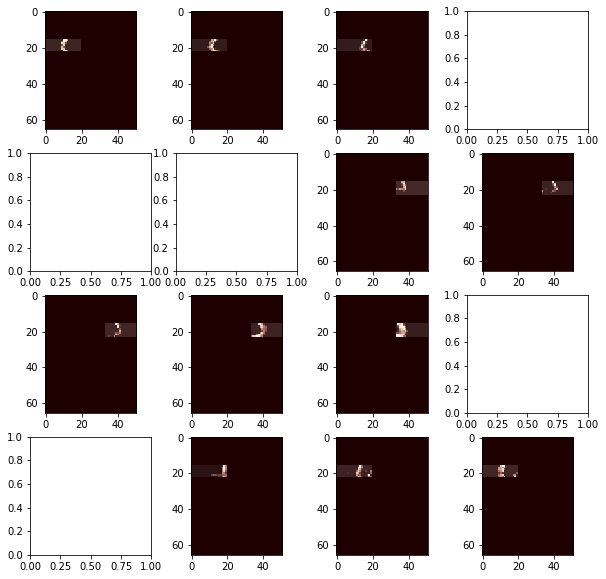
\includegraphics[width=4cm]{../Pic/cropped.png}
		\caption{A Crop result for region 4.(No image if this region is not shown in this angle)}
	\end{figure}
\end{frame}

%------------------------------------------------
\begin{frame}
\frametitle{Intuition: Multi-view CNN(MVCNN)\cite{su15mvcnn}}

	\begin{itemize}
		\item Used for 3D Shape recognition.
		\item Reported over 85 \% accuracy on ModelNet40.
	\end{itemize}
	\begin{figure}
		\centering
		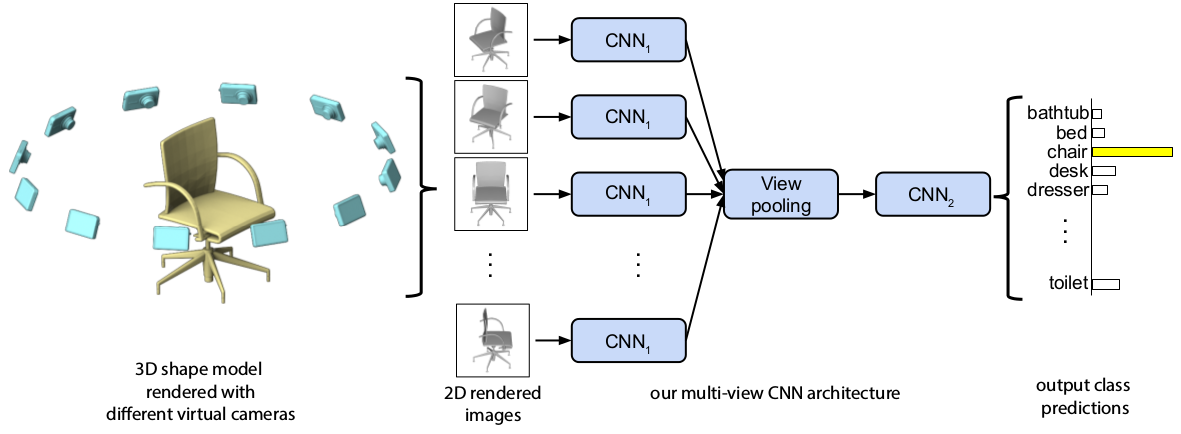
\includegraphics[width=10cm]{../Pic/mvcnn.png}
		\caption{A structure for MVCNN}
	\end{figure}

\end{frame}

%------------------------------------------------
\begin{frame}
\frametitle{Our Approach: MVCNN with attention}

	\begin{itemize}
		\item But our task is more tricky since the object may or may not be present, and it can be rather small compared to the main object in the image(human)
		\item Solution: Force attention
		\item 2D Convolution with kernel 1x1, 3x3 and 5x5 added to force attention on small areas.
		\item We maintain the size of the image after convolution and stack them together after 2D convolution.
	\end{itemize}

\end{frame}

%------------------------------------------------
\begin{frame}
\frametitle{Our Approach: MVCNN with LSTM attention}

	\begin{itemize}
		\item Intuition: 3 convolutions over a same region may report similar information.
		\item We add LSTM to network after stack all the convoluted images.(Now there is no more need to maintain size after 3 convolution.)
	\end{itemize}

\end{frame}


%------------------------------------------------
\begin{frame}
\frametitle{Stochastic Gradient Descent with Restarts(SGDR) \cite{SGDR}}

	\begin{itemize}
		\item Basic idea: \textit{Restart} learning rate after some time.
		\item Learning rate controlled by a cosine function whose cycle increases each time one cycle is reached. 
		\item It is reported that the error on CIFAR-10 and CIFAR-100 were 3.14\% and 16.21\% respectively\cite{SGDR}.
	\end{itemize}
	$$ \eta_t = \eta_{min}^i + \frac{1}{2}(\eta_{max}^i-\eta_{min}^i)(1 + \cos(\frac{T_{curr}}{T_i}\pi))$$
	$$ T_{i} = T_{i-1} * T_{mult} $$
	$T_0$, $T_{mult}$, $\eta_{min}^i$, $\eta_{max}^i$ is manually set.
\end{frame}

%------------------------------------------------
\begin{frame}
\frametitle{SGDR in Practice}

	\begin{itemize}
		\item We set $T_0$, $T_{mult}$ being 100 and 2 respectively.
		\item Others the same with the CosineAnnealingLR defined in pytorch
	\end{itemize}

\end{frame}

%------------------------------------------------
\begin{frame}
\frametitle{Our Approach: Filling Channels with Avg \& Std (Experimenting)}

	\begin{itemize}
		\item Observation: Anomaly appears when the data is either above or below average.
		\item Intuition: With average and stand deviation of a pose for all test samples provided, more accurate prediction should be possible.
		\item Practice: Put Avg in blue channel, Std in green channel and origin image in red channel.(resnet-50 needed 3-channel image anyway)
		\item Result: Still training.
	\end{itemize}

\end{frame}


%------------------------------------------------
\section{Experiment} % Sections can be created in order to organize your presentation into discrete blocks, all sections and subsections are automatically printed in the table of contents as an overview of the talk
%------------------------------------------------

%------------------------------------------------
\begin{frame}
\frametitle{Experiment: Network Structure}
	\begin{itemize}
		\item Criterion: BCEWithLogitsLoss()
		\item Optimizer: torch.optim.SGD
		\item Scheduler: SGDR
		\item 10 hours for 25 epochs.
	\end{itemize}
	\begin{figure}
		\centering
		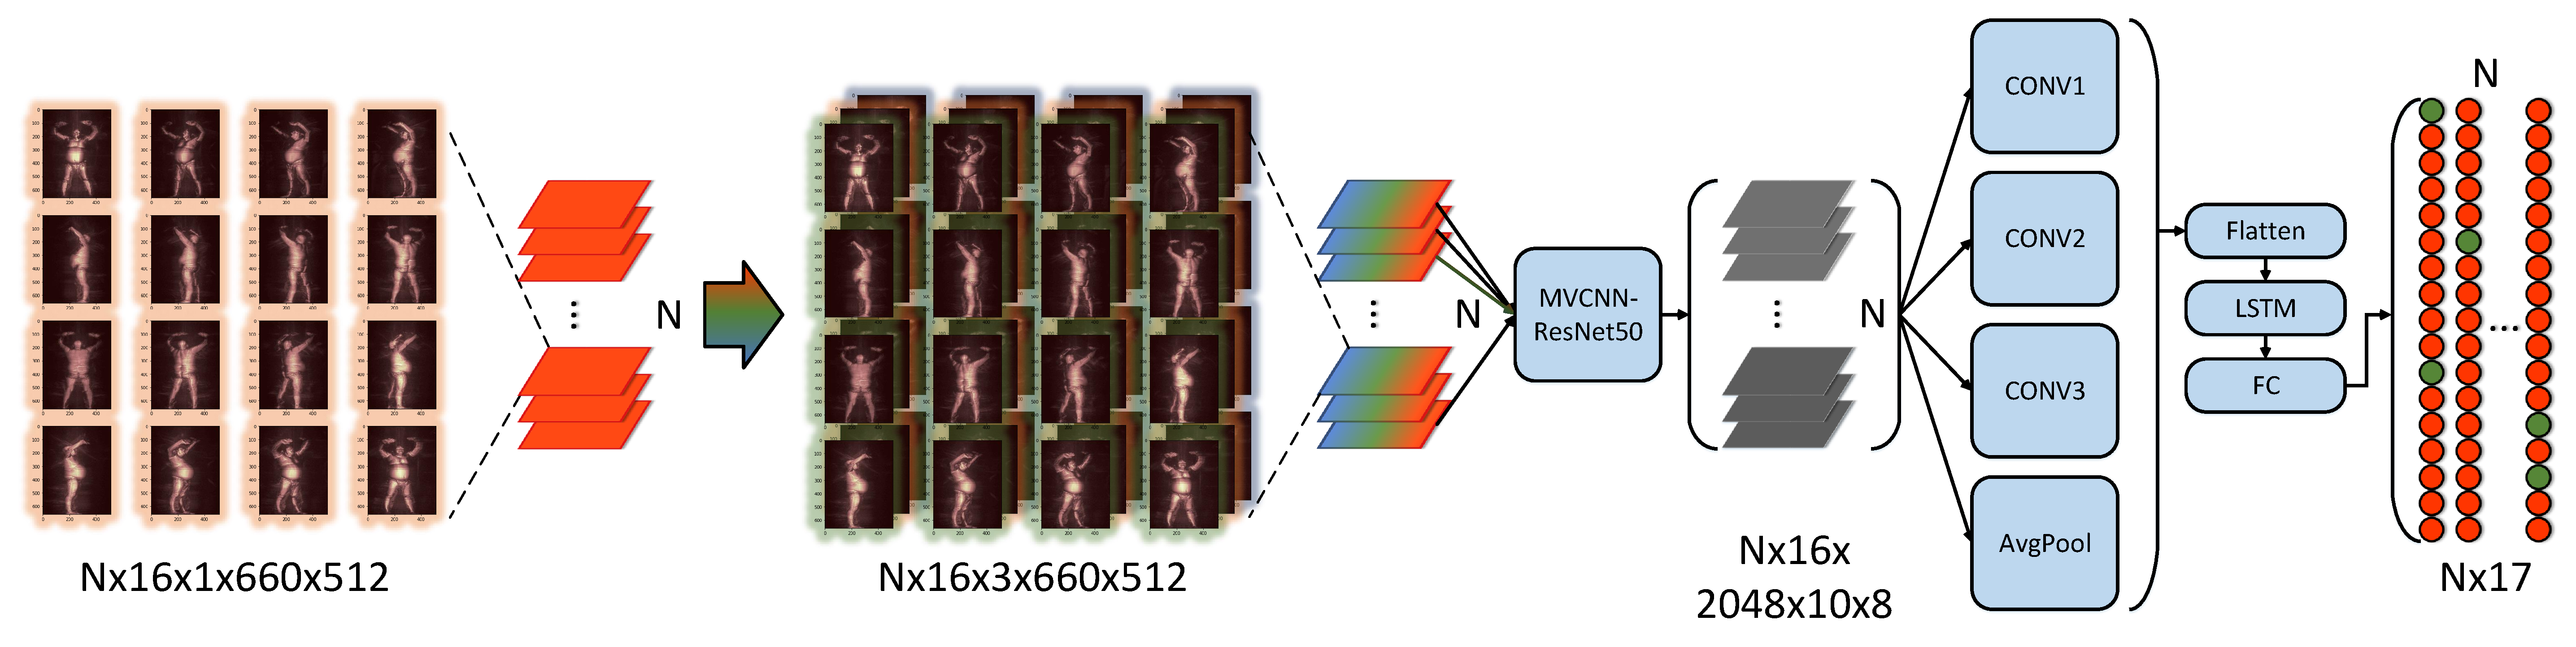
\includegraphics[width=12cm]{../Pic/Network.pdf}
		\caption{Our Network Structure.}
	\end{figure}

\end{frame}

%------------------------------------------------
\begin{frame}
\frametitle{Experiment Result: Attention Vs LSTM}

	\begin{figure}
		\centering
		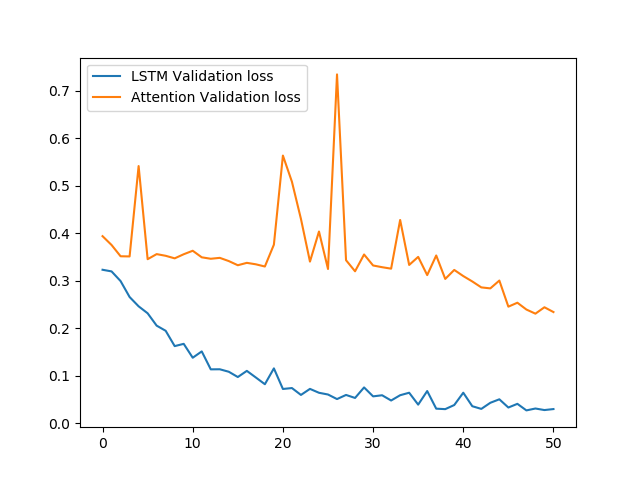
\includegraphics[width=10cm]{../Pic/2models.png}
		\caption{Different validation results.}
	\end{figure}
	
\end{frame}

%\begin{frame}
%\frametitle{Experiment Result: SDG Vs SDGR}

%	\begin{figure}%
%		\centering
%		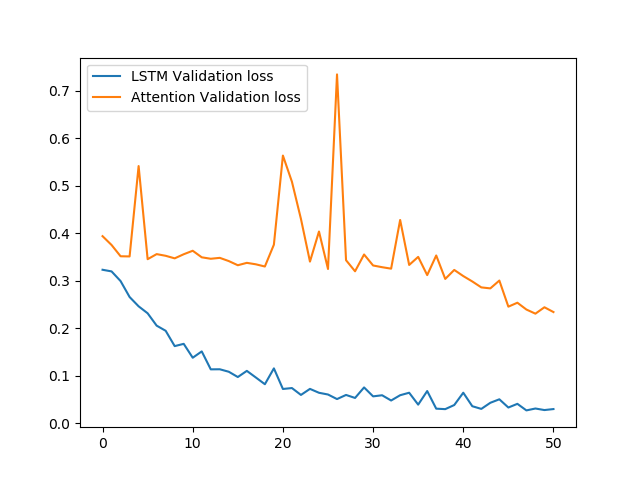
\includegraphics[width=10cm]{../Pic/2models.png}
%		\caption{SDGR Can be better.}
%	\end{figure}
	

%\end{frame}


%------------------------------------------------
\section{References} % Sections can be created in order to organize your presentation into discrete blocks, all sections and subsections are automatically printed in the table of contents as an overview of the talk
%------------------------------------------------

\begin{frame}
	\frametitle{References}
	\footnotesize{
		\begin{thebibliography}{99} % Beamer does not support BibTeX so references must be inserted manually as below
			\bibitem[Su, 2015]{su15mvcnn} Hang Su, Subhransu Maji, Evangelos Kalogerakis and Erik G. Learned{-}Miller (2015)
			\newblock Multi-view convolutional neural networks for 3d shape recognition
			\newblock \emph{Proc. ICCV}
		\end{thebibliography}

		\begin{thebibliography}{99} % Beamer does not support BibTeX so references must be inserted manually as below
			\bibitem[Loshchilov, 2016]{SGDR} Ilya Loshchilov and Frank Hutter (2016)
			\newblock {SGDR:} Stochastic Gradient Descent with Restarts
			\newblock \emph{CoRR abs/1608.03983}
		\end{thebibliography}
	}
\end{frame}
\end{document} 